\documentclass[lettersize,journal]{IEEEtran}
\usepackage{amsmath,amsfonts}
% \usepackage{algorithmic}
% \usepackage{algorithm}
\usepackage[linesnumbered, ruled]{algorithm2e}
\usepackage{array}
\usepackage[caption=false,font=normalsize,labelfont=sf,textfont=sf]{subfig}
\usepackage{textcomp}
\usepackage{stfloats}
\usepackage{url}
\usepackage{verbatim}
\usepackage{graphicx}
\usepackage{cite}
\hyphenation{op-tical net-works semi-conduc-tor IEEE-Xplore}
% updated with editorial comments 8/9/2021

\begin{document}

\title{{\huge CS303 Project 3 Report\\}{
Adult Census Income Classifier}}

\author{12111012 Kuang Liang}

\maketitle

\begin{abstract}
This document describes my work on CS303 project 3: Adult Census Income Classifier, containing the introduction of the problem, the choice of the module, the analysis process of the data and the reflect of the result.
\end{abstract}

\section{Introduction}

\IEEEPARstart{T}{he} Adult Census Income dataset is a census dataset released by the US Bureau of National Statistics that contains income information for over 1 million US adults, which is an important dataset used to study and analyze important social issues such as income distribution and wealth gap. In this project, part of the data was provided with their labels, and another part was provided without labels. Our target is to give those data without labels a prediction as accurate as possible.

\section{Module}

This problem is a binary classification problem with limited amount of data, many arguments and parts of them are non-numerical. We have many options for the module, such as decision tree, nearest neighbor classifier, support vector machine and neural network.

Nearest neighbor classifier is exculded first, because it cannot support high-dimension data well.

Decision tree seems to be the best solution, which is an understandable and explainable module with good performance, and also supports high-dimension data and non-numerical arguments. However, training a decision tree requires a large amount of data and time, but we only have about 20,000 records.

Support vector machine also seems to be a good idea with good performance on classification of high-dimension data. However, SVM requires data to follow approximate normal distribution, but we do not have this assumption. Meanwhile, SVM sometimes overfits seriously.

Therefore, I chose the neural network. Although the neural network has high complexity and poor interpretation, it has strong fault tolerance and an acceptable performance with limited data.

I learnt to train a neural network from the Internet\cite{ref1}. Its input layer has 13 nodes, hidden layer has 78 nodes and output layer has only one node. The activation function of hidden layer and output layer is ReLU and Sigmoid respectively. The loss function used is Binery Cross Entropy loss (torch.nn.BCELoss), and the optimizer used is Adam optimizer (torch.optim.Adam).

\section{Data}

In this part, I will introduce the data provided and how I processed it. Note that a small part of the data was missing and marked with a question mark.

\subsection{Composition of the data set}

\begin{itemize}
    \item{1.} Age (integer): the working age of each data sample, which is a numerical variable;
    \item{2.} Work class (string): type of work, where there are private, local government, etc., is a character type variable;
    \item{3.} Final weight (integer): the number of observational representatives of a sample in a state;
    \item{4.} Education (string): the level of education of each sample;
    \item{5.} Education number (integer): the schooling year of each sample;
    \item{6.} Marital status (string): marital status of each sample;
    \item{7.} Occupation (string): the occupation of each sample;
    \item{8.} Relationship (string): the family relationship of each sample;
    \item{9.} Race (string): the race of each sample;
    \item{10.} Gender (string): the sex of each sample;
    \item{11.} Capital gain (integer): a capital gain is a profit that results from a disposition of a capital asset, such as stock, bond or real estate, where the amount realised on the disposition exceeds the purchase price;
    \item{12.} Capital loss (integer): capital loss is the difference between a lower selling price and a higher purchase price, resulting in a financial loss for each sample;
    \item{13.} Hours per week (integer): sample weekly working hours;
    \item{14.} Native country (string): the country where the sample is from;
    \item{Output} Income ($\{0,1\}$, label): whether the income is greater than 50K or not.
\end{itemize}

\subsection{Analysis}

There are three types of arguments.

\begin{itemize}
    \item{1.} The most special argument: \textbf{3. final weight}, which means the weight of this sample, so it is not a characteristic of the sample.
    \item{2.} Numeric argument: \textbf{1., 5., 11., 12., 13.} which are all the integer arguments except 3., can be used directly in the analysis.
    \item{3.} String arguments: \textbf{2., 4., 6., 7., 8., 9., 10., 14.} which are string arguments, which cannot be directly transformed into numbers.
\end{itemize}

In my first attempt, I just ignored \textbf{3.}, and gave string arguments random values. To keep them the same in the training and testing, I simply assigned them to their length. I divided all of the data into 80\% for training and 20\% for testing, and achieved 76\% accuracy. However, when checking the result, I found that all outputs are 0 and the accuracy is actually the ratio of 0 over all testing data, so this attempt was completely a failure.

In this attempt, all the string arguments are just noise for the neural network, so it did not work well. I used pandas and matplotlib in python to analyze the data and draw some graphs. As \textbf{Fig 1.} showed, some string arguments, like 'native-country', can significantly affect the possibility of a higher income. Therefore, in my second attempt, I used this possibility to replace those string arguments, and now the neural network performed much better and achieved about 82\% accuracy.

After a little more attempts, I found the two arguments, \textbf{11. Capital gain} and \textbf{12. Capital loss}, are too uneven between different records. Most of them are 0, while others are extremely high. I tried to apply a simple function $f(x)=\ln(x+1)$ on them, and it reached 85\% accuracy immediately.

Finally, my neural network converged to accuracy 85\%, and with which I gave a prediction of the test data.

\section{Reflection}

According to an experiment on github\cite{ref2}, 85\% accuracy is an acceptable result on this dataset. However, I referred to many solutions on github during doing this project, but I did not manage to make use of 'fnlwgt' in the end. Meanwhile, I did not try multiple hidden layers and cannot explain the function used to process Capital gain and Capital loss.

\begin{figure}
    \centering
    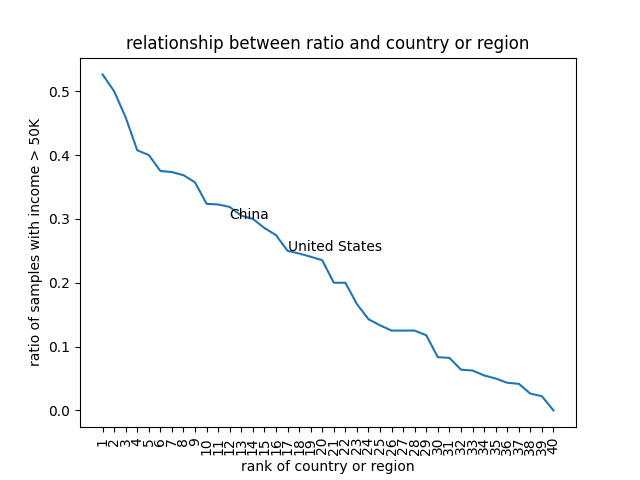
\includegraphics[height=6cm,width=8cm]{figure1.png}
    \caption{relationship between ratio and country or region}
    \label{fig1}
\end{figure}

\begin{thebibliography}{1}
\bibliographystyle{IEEEtran}

\bibitem{ref1} https://machinelearningmastery.com/develop-your-first-neural-network-with-pytorch-step-by-step

\bibitem{ref2} https://github.com/saravrajavelu/Adult-Income-Analysis

\bibitem{ref3} https://github.com/MorvanZhou/PyTorch-Tutorial/blob/master/tutorial-contents/302\_classification.py

\bibitem{ref4} https://github.com/UBC-MDS/Income-Predictors-for-US-Adults/blob/master/src/load\_data.py

\end{thebibliography}

\end{document}


